\documentclass[main.tex]{subfiles}
\begin{document}
\begin{enumerate}

\subsection{Section 4}

\item The magnetic field of a particular mode in a parallel-plate air waveguide with a plate separation of 2.5 cm is given by
$$H_{z}(x, y)=C e^{-j 640 \pi x / 3} \cos (160 \pi y)$$
where x and y are both in meters.
    
    \begin{enumerate}
        \item Is this a TE\textsubscript{n} or TM\textsubscript{n} mode? What is n? Is it a propagating or non-propagating mode?
        \item What is the operating frequency?
        \item Find the corresponding electric field.
    \end{enumerate}
    
\item An electromagnetic field in free space, $\mu_{0}=4 \pi \times 10^{-7}$ henry/meter, $\varepsilon_0 = 8.85 \times 10^{-12}$ farads/meter, is specified as by the vector phasor 

$$\underline{E}(\underline{r})=\underline{E}_{0} \varepsilon^{-j \underline{k} \underline{g} \underline{r}}$$

where $\underline{E}_{0}=\hat{x}$ the unit vector in the x direction of a rectangular coordinate system (x,y,z).

$$\begin{aligned}
&\underline{r}=x \hat{x}+y \hat{y}+z \hat{z} \\
&\underline{k}=-j \hat{y}+2 \hat{z}
\end{aligned}$$

    \begin{enumerate}
        \item What is the frequency f of the electromagnetic field (Hz)?
        \item Describe the equi-phase surfaces of the field. Write a general equation for the equi-phase surfaces.
        \item Describe the constant magnitude-of-field surfaces. Write a general equation for these equal-magnitude surfaces.
        \item Evaluate the average power as a function of position.
    \end{enumerate}

\item A plane wave is incident in the interface between two dielectrics $\varepsilon_1$ and $\varepsilon_2$, $\varepsilon_1 > \varepsilon_2$ as shown in figure \ref{fig:12q_a}.

\begin{figure}
\centering\fbox{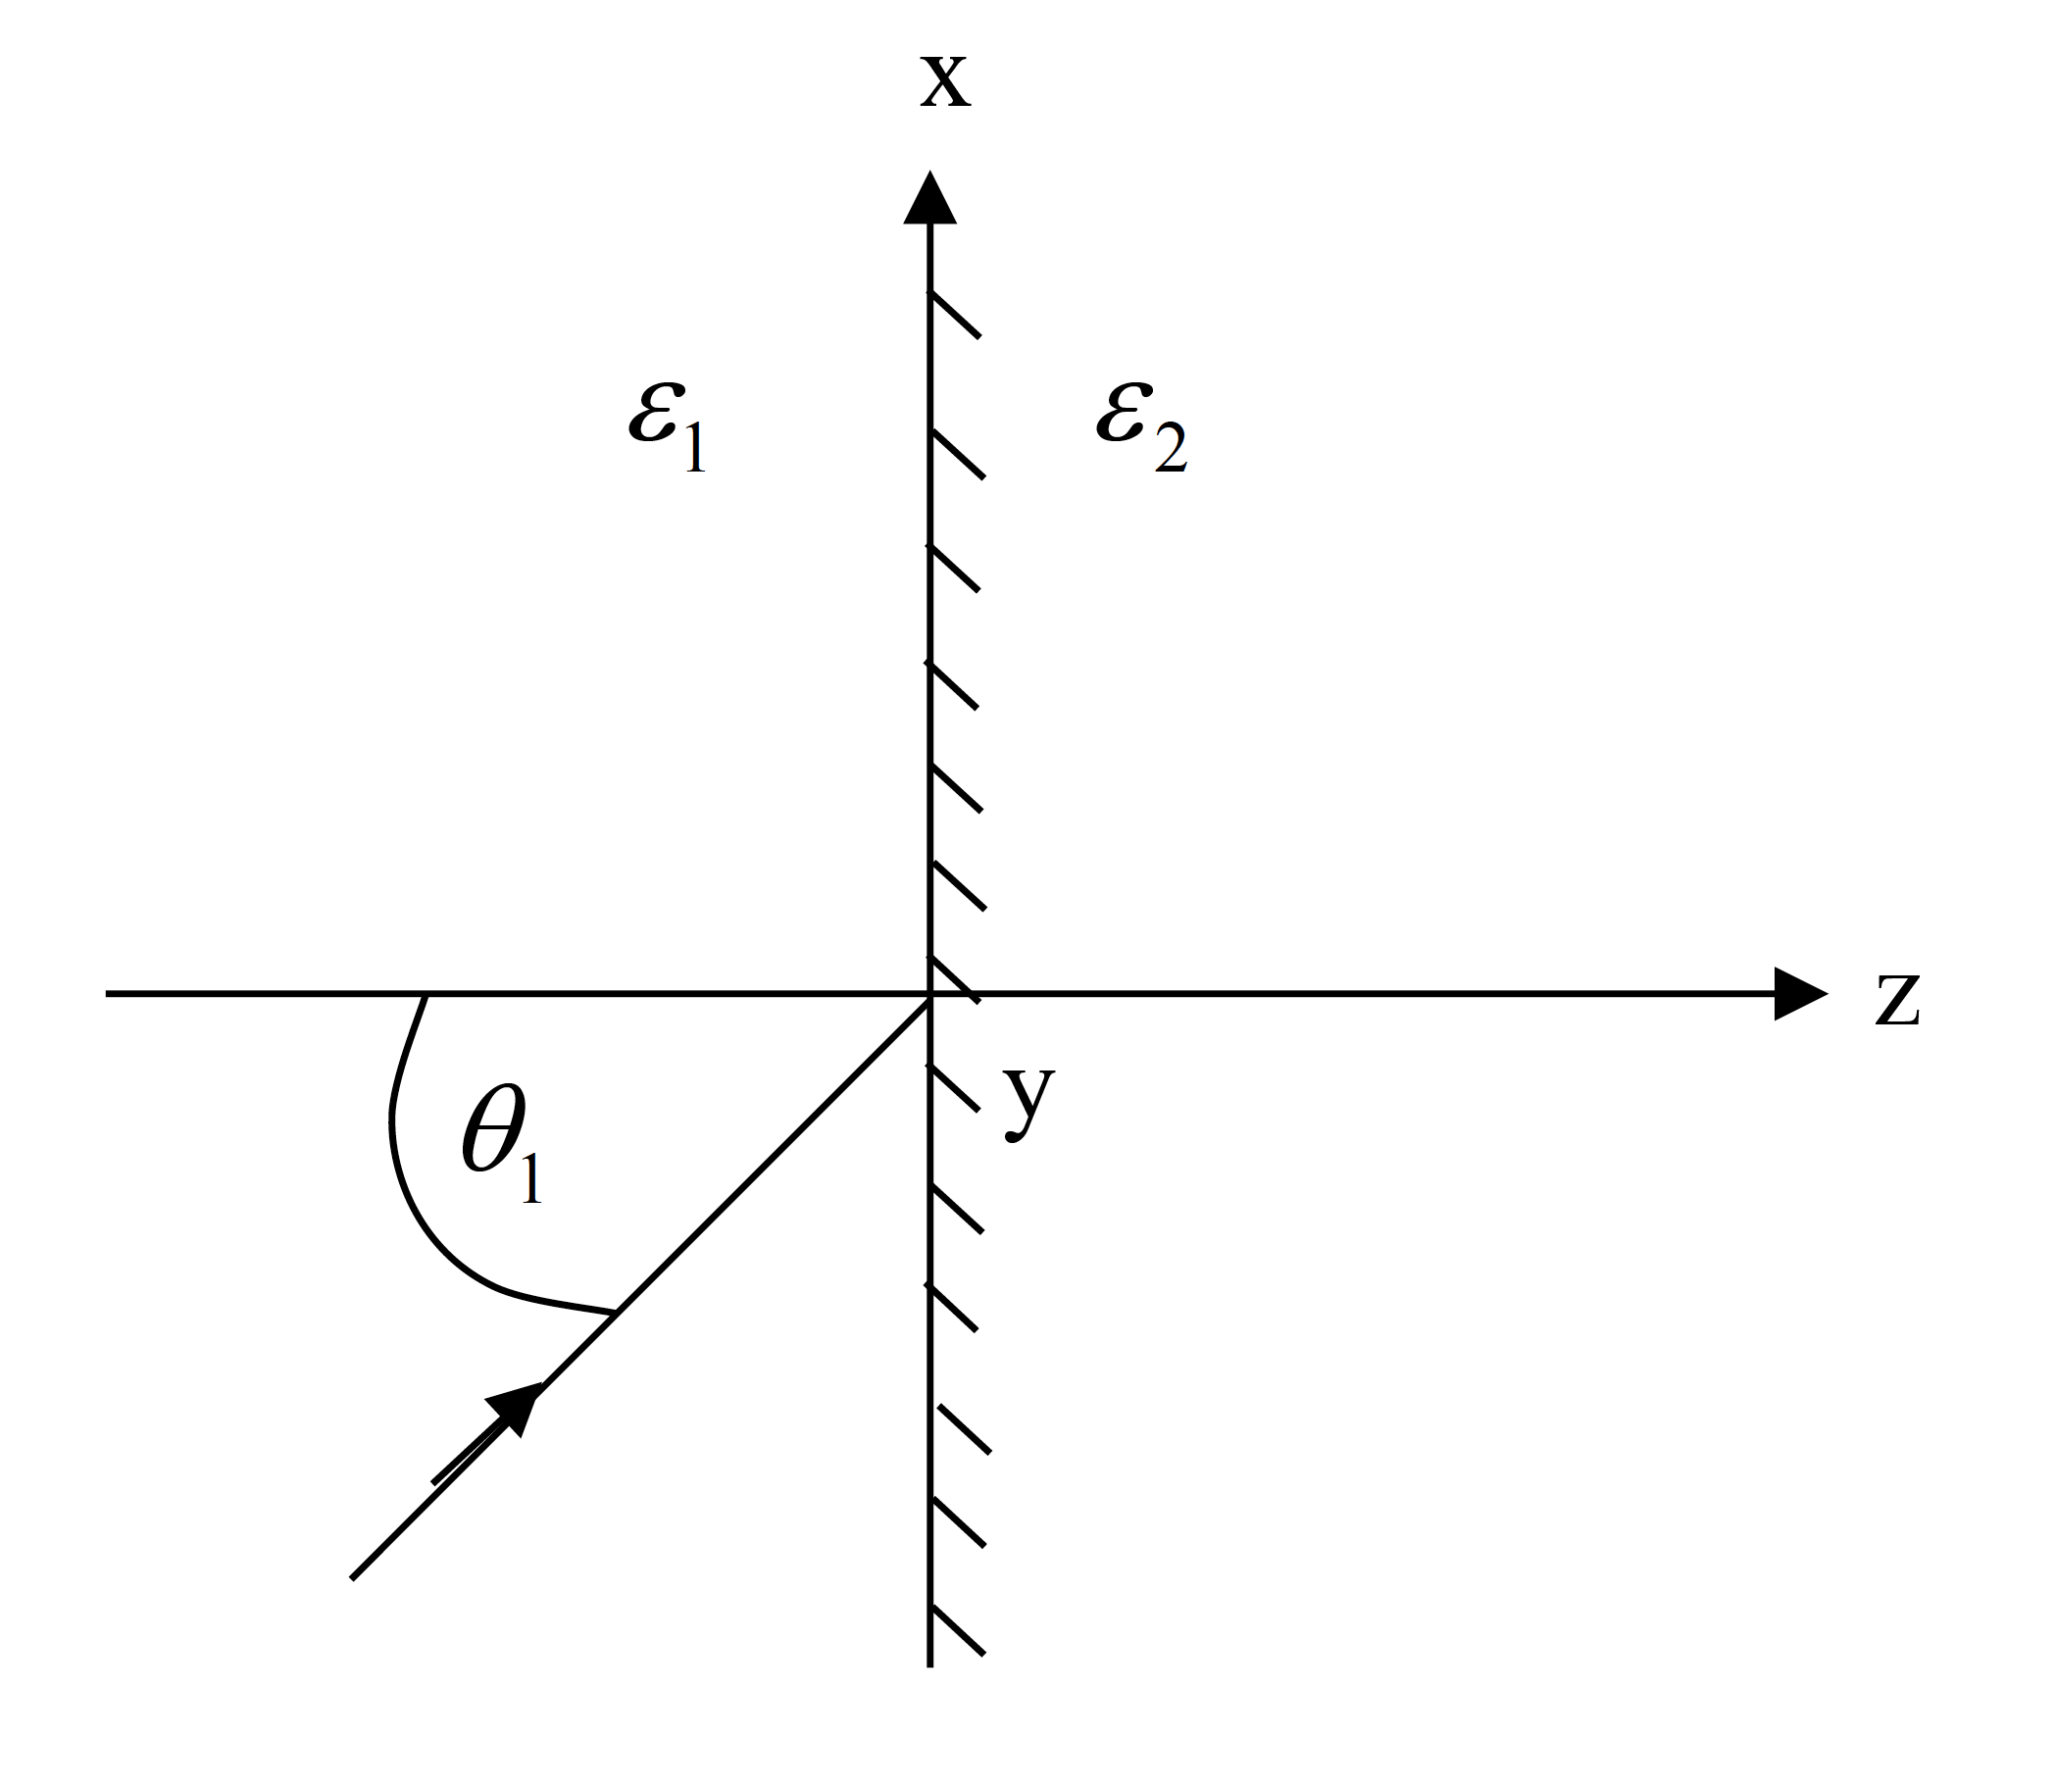
\includegraphics[width=2.0in]{figures/2018s/12q_a.png}}
\caption{Plane wave incident incident in the interface between two dielectrics}
\label{fig:12q_a}
\end{figure}

    \begin{enumerate}
        \item Find the angle $\theta_{1c}$ such that all waves incident with $\theta_1 > \theta_{1c}$ are "totally reflected".
        \item For $\theta_1 > \theta_{1c}$, describe the field (if any) in the region $z > 0$ in the $\varepsilon_2$ dielectric.
        \item If \underline{$E$} is perpendicular to the plane of the incidence, $\underline{E} = E_y \hat{y}$, find the phase of the reflection coefficient.
    \end{enumerate}

\end{enumerate}
\end{document}